
\section{How do skilled performers perform better on flat section in slalom?}


\subsection{Which strategies did the skiers perform best with?}
We begin by asessesing which of the four strategies—"stand against," "rock skis forward," "extend," and "extend with rock skis forward—yielded the best average performance for the skiers. To test this, we extracted the race times from the forced exploration session, where skiers in all groups tested all strategies. Since we accounted for practice order effects during this session by randomly assigning the test order of the strategies to each skier (under the condition that the first and last four trials included all four strategies), we could use these times to compare the effectiveness of each strategy.

To this end, we employed a Bayesian modeling approach (model 1) to estimate the expected differences between the strategies. The analysis revealed that skiers on average achieved their best descent times using the 'extend with rock skis forward' strategy (16.66 s, 95\% credible interval (CI) = 16.54, 16.77). The second best strategy for skiers was to step down to "extend" only, which was only 0.02 s (95\% CI = -0.02, 0.06) slower than the "extend with rock skis forward" strategy. However, when skiers switched from the "extend" strategy to the "rock ski forward" strategy, the expected time loss was 0.21 s (95\% CI = 0.16, 0.25). Finally, if the skiers switched from the "rock skis forward" strategy to the "stand against" strategy, the expected time loss was 0.2 s (95\% CI = 0.15, 0.25). Therefore, the strategies the skiers used made a great difference in race time.

These results show that just making clean, carved turns and resist the centripetal forces during a turn does not suffice to achieve fast race times on flat terrain in slalom. Instead, the active movements of the skiers were crucial for achieving fast race times on flats. When the skiers actively "rocked their skis forward", they improved their times greately compared to "stand against" only. This finding aligns well with prior findings in slalom skiing that reported a strong correlation between fore and aft movements and energy dissipation, such that more fore movements were associated with greater energy dissipation \cite{reid_turn_2009, reid_kinematic_2010}. Furthermore, studies have shown that faster skiers have a greater range of fore/aft motion and spend a larger portion of the turn skiing with their weight shifted back after gate passage than slower skiers \cite{tjorhom_beskrivelse_2007, reid_kinematic_2010}. Our results extend these findings and provide experimental evidence that "rock skis forward" can be an effective strategy for improving race times on flat terrain in slalom.

The 'rock skis forward' strategy resulted in much slower times than did the 'extend' strategy, however. Predictions from the Lind and Sanders model \cite{lind_physics_2013} indicate that extending the center of mass closer to the axis of rotation during a turn from a laterally inclined position should significantly improve the race time. Without motion capture data, we cannot assess the extent to which skiers extended and the resulting increase in kinetic energy. Nonetheless, the results suggest that skiers' extension movements play a crucial role in slalom performance, contrary to previous beliefs \cite{supej_differential_2008, supej_doba_2001}.

Finally, we found that "extend with rock skis forward" on average was the best strategy. This finding aligns with previous simulations suggesting that this strategy is most effective when skiers pump over rollers \cite{mote_accelerations_1983} and that it can be transferred to skiers executing a turn \cite{reid_kinematic_2010}. However, it is important to emphasize that "extend with rock skis forward" only was marginally better than the "extend" strategy alone. One reason for the limited improvement achieved by adding "rock skis forward" to the "extend" strategy might be that rocking the skis forward during the turn compromised how much the skier could extend toward the turn's axis of rotation. For instance, extensive extension could be challenging if the skier's center of mass was located at the tail of the skis. This issue should be further investigated in future analyses.

One limitation of these timing analyses is that we do not have precise knowledge of how much the skiers moved when executing the strategies or how these strategies affected the mechanical energy during a turn. Therefore, we cannot comment on the skiers' actual execution or the energy mechanics behind each strategy. Future studies should incorporate motion capture to address this gap in understanding.


\begin{figure}[H]
\centering
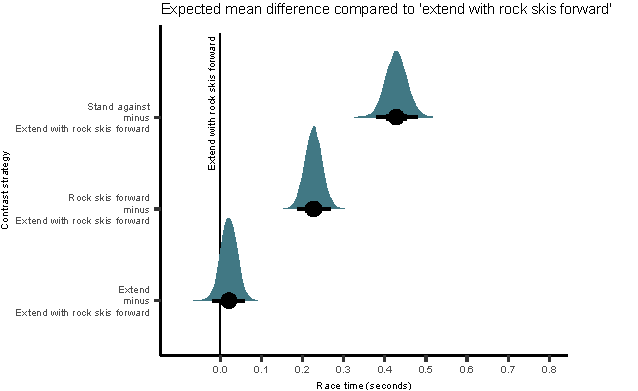
\includegraphics{figure/figure_results_Q1_strategies_2.pdf}
\caption{Expected differences in means compared to 'extend with rock skis forward' (that is, the expected best strategy). The circle represents the point estimates whereas the shaded distribution represents the expected posterior of the mean differences from the model.}
\label{fig:q1_strategieseffect}
\end{figure}



\subsection{LPS}
From the previous section, we learned that the 'extend' strategy was effective and nearly as efficient as the 'extend with rock skis forward' strategy. In Study 2, skiers significantly improved their race times after a three-day training intervention focused solely on the 'extend' strategy. Our next aim was to examine the kinematic changes that occurred during this intervention to understand what the skiers learned or did differently. Since race time in alpine skiing depends on speed and path length, these kinematic changes could manifest as alterations in either speed or path length. We investigated which of these changes were most consistent with the data and whether the kinematic changes aligned with the mechanical theory of pumping. To explore this, we used recording data from a small segment of the slalom course and a subset of skiers (18 out of 66) for whom we had set up a local positioning system in the rest of the slalom course. This allowed us to quantify both path length and instantaneous speed.

If the pumping mechanism drove the skiers' improvement in race time, we would expect skiers to increase their speed at or immediately after gate passage, at the time when the extension movement occurs. Fig. \ref{fig:lps_speed}a shows the speed profiles for the local positioning system section during baseline and retention. We first describe the average speed trend at baseline and then the contrast between baseline and retention.

In the baseline test, the skiers’ speed decreased for each gate in the local positioning system section compared to their speed during straight gliding, except for a slight speed increase of 0.05 m/s (95\% CI[-0.08, 0.17]) from gate 1 to gate 2. In the other gate sections, the speeds decreased on average by -0.06 m/s (95\% CI[-0.19, 0.07]) from gate 2 to gate 3 and by -0.12 m/s (95\% CI[-0.25, 0]) from gate 3 to gate 4 compared to straight gliding times. We report only the comparisons at the gates because the gates mark a fixed reference point. After the training intervention, the skiers increased their entry speed into the local positioning section (gate 1) by an average of 0.24 m/s (95\% CI [0.19, 0.29]) compared to the baseline speed. From this gate, the skiers tended to increase their speed throughout the section. Specifically, the skiers increased their speed on average by 0.07 m/s (95\%CI [0.01, 0.12]) from gate 1 to gate 2, followed by a slight decrease of -0.02 m/s (95\%CI [-0.05, 0.02]) from gate 2 to gate 3. Subsequently, the speed of the skiers increased again by 0.1 m/s (95\% CI[0.06, 0.14]) from gate 3 to gate 4. Therefore, the speed of the skiers increased almost incrementally from gate to gate. In addition, the speed profiles appeared wavier, as depicted in Figure \ref{fig:lps_speed}b. In general, the pattern of these waveforms was that skiers increased their speed after gate passage and continued to rise until the skiers were approximately midway between two gates. After that, the speed decreased to the gate before it rose again. As such, the speed profile changed massively from baseline to retention. 

\begin{figure}
    \centering
    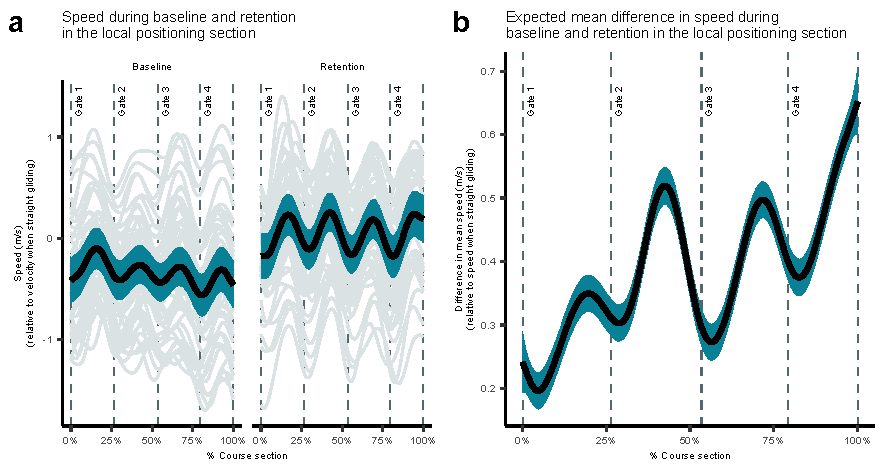
\includegraphics[width=1\linewidth]{figure/figure_speed.pdf}
    \caption{Enter Caption}
    \label{fig:lps_speed}
\end{figure}


Next, we analyzed the path length, for which we did not expect would undergo big changes based on the recording system we used. At the baseline test, we found that the total path length from gate 1 to gate 2 was 10.00 m (95\% CI[9.97, 10.10]), 10.7 m (95\% CI[10.70, 10.80]) from gate 2 to gate 3, and 10.10 m (95\% CI[10.10, 10.10]) from gate 3 to gate 4, while it was 8.19 m (95\% CI[8.15, 8.23]) from gate 4 to the end of the section. Notably, the reason for the lower estimate from gate 4 to the end is that this section was shorter than the other gate sections because the section ended before gate 5. Figure 5 panel a shows the total path length during each gate in the local positioning system section. Overall, we found no clear systematic differences in path length from baseline to retention across the gates. Surprisingly, the expected mean difference was 0.17 m (95\% CI[0.06, 0.28]) longer from gate 1 to gate 2 in retention. This expected mean difference did not overlap with the baseline estimate. Conversely, the expected mean difference overlapped considerably between baseline and retention for gate 2 to gate 3 (-0.02 m, 95\% CI[-0.14, 0.10]) and for gate 3 to gate 4 (0.02 m, 95\% CI[-0.02, 0.06]). In contrast, we observed an increased path length in retention from gate 4 to the end of the section (0.08 m, 95\%CI[0.04, 0.13]). In summary, we found changes in path length for some gate sections, while others showed minor differences. The general trend was that the skiers skied a longer path length during retention than at baseline. Figure 5b illustrates the expected mean difference in total path length for each gate in the local positioning section 

Our data indicate that the intervention led to an increase in speed and path length in certain gate sections. How does this align with previous alpine research and mechanical theories on pumping? First, these and previous results suggest that the 'extend' strategy (or pumping) might significantly impact athletes' performance in flat sections, contrary to previous beliefs \cite{supej_differential_2008, supej_doba_2001}. The increased speed from turn to turn and the distinct change in the speed profile align well with expectations from a pumping mechanism to increase the speed from turn to turn. We also observed a trend where the path length increased slightly from gate to gate, although this varied significantly from turn to turn. Several factors could explain this increased path length, which we cannot quantify or separate using the local positioning system. One possibility is that pumping increases the path length because the extension movement exerts more force on the skis, causing them to bend and turn more. However, this could also result from measurement errors from the local positioning systems or differences in the course setting.


\begin{figure}
    \centering
    \includegraphics[width=1\linewidth]{figure/figure_path.pdf}
    \caption{Enter Caption}
    \label{fig:lps_speed}
\end{figure}




To conclude, we found that the skiers' speed profiles underwent significant changes, consistent with the changes we would expect from pumping. We also found that the skiers tended to ski a longer path at the retention session, yet they accomplished better descent times. However, it is important to consider the limitations of this study, which we discuss further in the methodological section. 

\section{Using contextual interference to create challenging problems for skiers did not improve perfor}
Our next question was whether coaches can leverage contextual interference to design challenging learning problems to improve learning. Skiers trained to pump on flat sections in slalom either in one course per day (blocked practice) or in different courses randomly assigned each day (interleaved practice). Based on the typical results of the contextual interference effect \cite{simon_metacognition_2001, shea_context_1983, hall_contextual_1994, shea_contextual_1979, tsutsui_contextual_1998, thomas_using_2021}, we hypothesized that the blocked learning group would perform better during the training sessions (acquisition) than the interleaved learning group because they repeatedly skied on the same course and therefore could perfect their performance on this course before switching to the next (thus experiencing less interference). During the first four trials (trial block 1), we found no statistically significant differences between the interleaved and blocked practice groups on course A ($\beta$ = 0.17, 95\% CI[-0.19, 0.53], $t$(91.971) = 0.95, $p$ =  0.344), course B ($\beta$ = -0.03 , 95\% CI[-0.38, 0.33], $t$( 91.241 ) = -0.14, $p$ = 0.886) or course C ($\beta$ = 0.14 , 95\% CI[-0.21, 0.5], $t$(92.069) = 0.81, $p$ = 0.421). Both learning groups improved their race times over the subsequent trial blocks (blocks 2 and 3)(Supplementary Table \ref{paper1: racetimechangepercourse}). However, we found no statistically significant greater improvement in the blocked practice group for any course (Supplementary Table \ref{paper1: racetimeinteraction}). The differences between the learning groups in trial block 2 or trial block 3 were also not statistically significant (Supplementary Table \ref{paper1: racetimedifferencebetweentreatments}). Fig \ref{fig:enter-label})a shows the mean race time estimates for the three trial blocks during acquisition for the three courses. Based on these findings, we did not find evidence that the blocked learning group improved more during the training sessions than the interleaved learning group. 

Our second hypothesis was that the interleaved learning group would outperform the blocked learning group on the retention test conducted after a three-day retention interval. However, we found no evidence against the null hypothesis of no difference between learning groups for course A ($\beta$ = 0.09, 95\% CI[-0.12, 0.3],$t$(45.131) = 0.89 , $p$ = 0.379), B ($\beta$ = 0.13, 95\% CI [-0.18, 0.44], $t$(45.566) = 0.85, $p$ = 0.397), or C ($\beta$ = 0.05, 95\% CI [-0.29, 0.39], $t$(44.813) = 0.29, $p$ = 0.772). Therefore, we found no convincing evidence that the interleaved learning group improved retention.

\begin{figure}
    \centering
    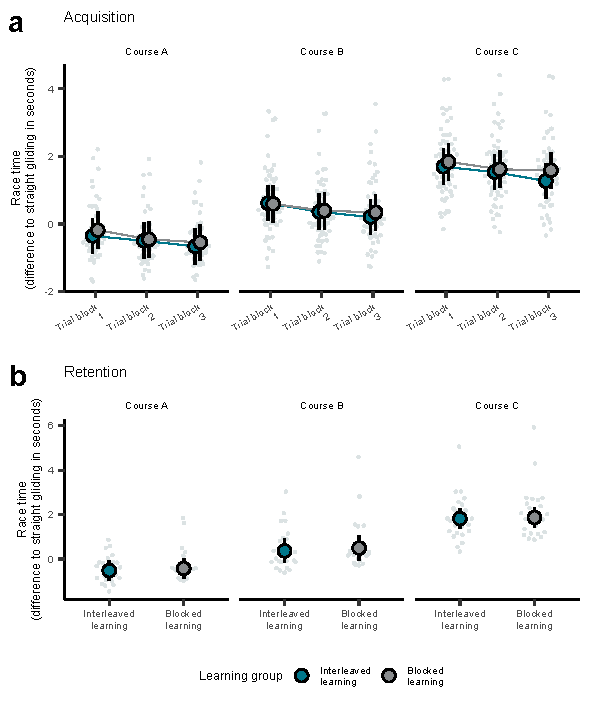
\includegraphics[width=1\linewidth]{figure/figure_results_ci_acquisitionandretention.pdf}
    \caption{Enter Caption}
    \label{fig:ci_results}
\end{figure}

To begin, our study aligns with previous research that has not found a contextual interference effect in real-world tasks or more complex activities \cite{brady_theoretical_1998, barreiros_contextual_2007, wulf_principles_2002}. One reason for this is that the skiers were skilled, and the sport is complex. A comparable study revealed no significant effect of frequent task switching (alternating between two types of serves in the interleaved learning group) on learning tennis serves among younger players\cite{buszard_quantifying_2017}. However, the tennis players in this interleaved learning group improved their serves in competition (transfer) compared to those in the blocked learning group. In contrast, \cite{hall_contextual_1994} found that baseball players batted better after training with interleaved learning over several weeks than after training with blocked learning. The key difference between these two studies is that the former manipulated contextual interference between two different skill types, while the latter manipulated variations of the same skill. Therefore, the way the manipulation was performed (between skills versus between variations of one skill) might be a contributing factor. However, our study is most consistent with the manipulation type in \cite{hall_contextual_1994} study and should have corroborated the findings from that study. Therefore, it appears that this is not the best explanation for our data.

Another reason for the difference in results between our study and previous studies on contextual interference is that skiing is a continuous skill, while most of the literature focuses on learning discrete skills\cite{lee_distribution_1988, lee_distribution_1989}. Although contextual interference has been found for continuous tasks\cite{pauwels_contextual_2014, tsutsui_contextual_1998}, these findings come from beginners and relatively simple tasks. According to the 3R framework of motor learning \cite{tsay_strategy_2023}, skilled performers are adept at recognizing changes in the learning environment and quickly adapt their control policy to improve performance if a better alternative exists. Therefore, the skiers in the interleaved learning group may not have experienced significant interference because they quickly identified the new task and quickly switched to a more effective control policy. Since ski runs endure over a long time, skiers could adjust their control policy within the first few gates without significantly compromising their performance.

A third potential counteracting factor of the contextual interference effect in our study was the long rotation time between each run, which may have contributed to forgetting. Skiers took approximately 8 minutes between trials to ride the lift to the top and prepare for a new run. This intertrial interval is significantly longer than those used in laboratory tasks with discrete tasks \cite{barreiros_contextual_2007}. The extended time between trials might have caused skiers to forget and lose connections between trials, which is a mechanism suggested to underlie the contextual interference effect \cite{lee_locus_1983, lee_can_1985}. This perspective also aligns with the new theory of disuse \cite{bjork_new_1992}, which posits that lengthening the spacing between trials can increase forgetting yet enhance learning by reducing memory retrieval strength before each trial. Thus, both the interleaved and blocked groups might have experienced favorable learning conditions for skill learning due to the long intertrial.

Although we did not find significant differences between the learning groups, this does not imply that we do not recommend coaches frequently switch courses to create learning problems for skiers. Our findings only suggest that within the short duration of our training study (equivalent to a typical ski camp), we found no convincing benefits of interleaved learning. However, an important general training principle is the specificity principle \cite{lee_chapter_1988}, which states that training should meet the demands of the sport. In alpine skiing, skiers constantly encounter new competition courses, making it crucial for training to cover this range of variation. Frequently changing courses could help avoid the formation of undesirable habits \cite{du_relationship_2022}, such as skiers learning a solution to a situation only by perfecting it on a single course. While our study did not provide data to support this, it is a potential area for future research.

One limitation of this study is that the interleaved and blocked learning groups trained together, which could have created some treatment diffusion when the skiers observed each other from the lift or the top of the course. Unfortunately, we were unable to control for this potential limitation in this study due to space and time constraints in the ski hall. Another limitation is the absence of a transfer test, which could have provided important insights into the learning groups’ adaptation to a new slalom course.

To conclude, we did not find convincing evidence that coaches could leverage contextual interference to design challenging learning problems to improve learning.

\section{Using reinforcement-guided teaching signals improved training and performance compared to supervised-guided teaching signal}
The final question of this doctoral study addressed which teaching signal is most effective for teaching skiers to make optimal strategic choices, thereby impacting their performance and learning. In our learning experiment, skiers learned the value of different strategies through two main teaching strategies. One learning group used reinforcement learning, where skiers chose strategies themselves and evaluated their chosen strategy based on their race time. The other learning group used supervised learning, where a coach instructed them on which strategies to use. In the supervised (target skill) learning group, coaches always chose the theoretically optimal strategy and therefore served as a benchmark for the best possible strategy and performance. In the supervised (free choice) learning group, coaches selected the strategy they believed would be most beneficial for the skier to use.

\begin{figure}
    \centering
    \includegraphics[width=1\linewidth]{figure/figure_racingtimes_2.pdf}
    \caption{Race time across the different sessions for the three learning groups \textbf{a}. Estimated race times during the three acquisition sessions. Forced exploration refers to the sessions wherein skiers tried all strategies, whereas free choice 1 and free choice 2 refer to the session wherein skiers or coaches selected strategies according to their assigned learning groups. \textbf{b.} Estimated race times for retention. \textbf{c.} Estimated race times for transfer. Intervals represent the 95\% confidence intervals (CIs) derived from the models. Asterisks (*) indicate a statistically significant effect. Each light gray point represents a single trial performed by a skier.}
    \label{fig:rlstudy_racetime}
\end{figure}

To begin, we expected the reinforcement learning group to improve their race time more during the three acquisition sessions than did the supervised (target skill) learning group. We hypothesized that this improvement would result from better learning to select effective strategies. However, we did not expect the reinforcement learning group to select better strategies than the supervised (target skill) learning group. The skiers in this group were instructed to choose the optimal strategy and therefore served as a benchmark for the maximum expected benefit of improved strategy selection through reinforcement learning. First, we analyzed differences between the learning groups during the forced exploration acquisition session, where all groups were required to try all strategies. Therefore, we did not expect to find differences between the groups at this session. The results confirmed our expectations; we found no statistically significant differences between the reinforcement learning group and the supervised (free choice) learning group ($\beta$ = 0.06, 95\% CI [-0.2, 0.32], $t$(92.727) = 0.48, $p$ = 0.631), or between the supervised (target skill) learning group  ($\beta$ = 0.18, 95\% CI[-0.08, 0.44], $t$(92.663) = 1.37, $p$ = 0.174).  

To allow the learning groups to choose their own strategies-skiers in the reinforcement learning group and coaches in the two supervised learning groups-during the next two sessions in acquisition (free choice sessions 1 and 2), we expected the learning groups to show the development patterns outlined above. First, we observed that all learning groups significantly improved their race times over the course of the free choice sessions during acquisition (Supplementary Table \ref{table_racetime_acquisition_change}). The improvements across these sessions indicate that the choice of strategies exerted a great influence on race time in all the learning groups. However, consistent with our expectations, the three learning groups developed differently. The supervised (target skill) learning group, where skiers were coached to select the theoretically best strategy, showed a statistically significant greater improvement than the reinforcement learning group from forced exploration to free choice 1 ($\beta$ = -0.12, 95\% CI[-0.22, -0.03], $t$(91.777) = -2.58, $p$ = 0.012). Conversely, the supervised (free choice) learning group demonstrated a descriptively poorer progression than the reinforcement learning group, although this difference was not statistically significant ($\beta$ = 0.08, 95\% CI[-0.02, 0.17], $t$(92.5) = 1.61, $p$ = 0.110). Continuing this trend, comparing initial performance during forced exploration to performance in the final acquisition session (free choice 2), the reinforcement learning group improved significantly more than the supervised (free choice) learning group did ($\beta$ = 0.14, 95\% CI[0.02, 0.26], $t$(95.743) = 2.26, $p$ = 0.026). For the same comparison, the supervised (target skill) learning group no longer showed significantly greater improvement than the reinforcement learning group  ($\beta$ = 0.02, 95\% CI[-0.11, 0.14], $t$
(95.651) = 0.26, $p$ = 0.798). This is due in part to the continued improvement of the reinforcement learning group but also to a descriptive decline from free choice 1 to free choice 2 in the supervised (target skill) learning group, attenuating their initially greater improvement rate. However, we did not find statistical evidence that the reinforcement learning group performed better than the supervised (free choice) or supervised (target skill) learning groups at free choice 1 or free choice 2 (Supplementary Table \ref{table_racetime_acquisition_groupdifference}). Fig. \ref{fig: racetime}a presents the mean race time estimates during the three acquisition sessions. 

In the retention session, the skiers independently chose their strategies, irrespective of their assigned groups. We reasoned that at this point, the reinforcement learning group had learned to understand which strategies were most effective and chose them. Therefore, our hypothesis was that the reinforcement learning group would outperform the supervised (free choice) learning group in retention due to better strategy selection learned from observing the race times to evaluate the strategies. Consistent with this hypothesis, we found that the reinforcement learning group performed significantly better than the supervised (free choice) learning group did ($\beta$ = 0.12, 95\% CI[0.01, 0.24], $t$(101.422) = 2.12, $p$ = 0.037). The difference between the reinforcement learning and supervised (target skill) learning groups also favored reinforcement learning but was smaller and not statistically significant  ($\beta$ = 0.07, 95\% CI[ -0.04, 0.19], $t$(101.63) = 1.27, $p$ = 0.206). We therefore provide evidence that the reinforcement learning group performed better at retention than did the supervised (free choice) learning group. Descriptively, the reinforcement learning group performed better, even than the supervised (target skill) learning group, which served as an upper bound reference. Fig. \ref{fig: racetime}b presents the mean race time estimates during retention. 

Vår hypotese var at den forbedrede prestasjonen til reinforcement learning gruppen sammenlignet med supervised (free choice) var drevet av bedre strategivalg fordi de fikk muligheten til learning the strategies' values directly from observing race times. We testet denne hypotesen ved å teste om reinforcement learning gruppen utviklet en greater sannsynlighet for å velge den teoretiske beste strategien ("extend with rock skis forward") og den individuelle utøveres estimerte beste strategi. We did not find corroborating evidence for this hypothesis with any of these tests, however. I stedet støttet dataen vår to andre forklaringer på denne prestasjonsforbedringen. First, we found that the skiers in the reinforcement learning group who made 'suboptimal' choices during the retention session had a lower 'cost'-the expected the difference between a suboptimal chosen strategy and the skier's estimated best strategy-for their choices than did the skiers in the supervised (free choice) learning group. The reinforcement learning group therefore appears to have learned to select strategies that offered comparable outcomes and to avoid those that carried the risk of substantially worse performance. Second, we found that the reinforcement learning group improved more on the 'extend' strategy over the course of the sessions than did the supervised (free choice) learning group. One possibility is that the reinforcement learning group discovered that the "extend" strategy alone almost provided full benefits on its own and chose this strategy because it was simpler than "extend with rock skis forward" and subsequently refined this strategy. Jeg har valgt å ikke ta med figurer eller resultater i dette i denne thesis på grunn av plassbegrensninger. For fullstendige resultater og diskusjon, se paper 3. 

Våre resultater viser at reinforcement learning kan være en effektiv teaching strategi for å forbedre trening og prestasjon hos gode utøvere. Den estimerte gruppeforskjellen var også betydelig og kan utgjøre en forskjell på utøveres ferdighetsutvikling. If we assume that a full slalom course of approximately 45 seconds has a flat section equivalent to approximately 15 seconds (quite normal) and that a slalom race consists of two runs, the 0.12-second difference can translate into an improved Fédération Internationale de Ski (FIS) world ranking of 27 positions for females and 65 for males, based on a median ranking of 600 in our sample (see Supplement Discussion \ref{supdiscussion}). Det er likevel greit å notere seg at den estimerte effekten likevel mindre enn vår smallest effect size av interesse, hvilket var et benchmark som ble satt for andre betingelser enn vi klarte å gjennomføre på grunn av tids- og plassbegrensninger i skihallen. 

One limitation of the study is that we did not use motion capture to analyze the skiers' execution of the strategies. Consequently, we cannot describe the actual execution of the strategies, except that they were able to perform the strategies during the familiarization test. However, taking into account execution might have led to explosion of actually implemented strategies that would then be difficult to study. Yet, it is likely that the reinforcement learning group learned not only on the strategy level but also along an execution level that we were not able to quantify in this study.









\subsection{Race times}\label{result_racetime}
We assumed that the strategy choice would greatly impact race time in the slalom course and that the reinforcement learning group would learn to select better strategies and consequently perform better over the course of the experiment compared to the supervised (free choice) learning group where we used the skiers' own coaches. The supervised (target skill) learning group was instructed to choose the optimal strategy and therefore served as a benchmark for the maximum expected benefit of improved strategy selection through reinforcement learning. As our first step, we analyzed whether the learning groups showed pure time differences across the different sessions without taking the chosen strategy into account. 

\subsubsection{Greater performance improvement for  reinforcement learning  compared to supervised (free choice) learning}\label{result_racetime_acquisition}
If the reinforcement learning group learned to select better strategies than the supervised (free choice) learning group, we would expect them to exhibit greater improvement over the course of the three acquisition sessions. Therefore, our hypothesis was that the reinforcement learning group would improve more during the acquisition sessions than the supervised (free choice) learning group. Further, we would expect the supervised (target skill) learning group to rapidly improve race time when the skiers were instructed to only select the theoretical best strategy during the last two acquisition sessions (free choice 1 and free choice 2). 
We expected that differences in improvement between the learning groups would emerge once the skiers or the coach had the autonomy to pick the strategy over the course of the second (free choice 1) and third (free choice 2) acquisition sessions. Importantly, the three learning groups performed similarly during the forced exploration where they had the same number of trials on each strategy; we found no statistically significant differences between the reinforcement learning group and the supervised (free choice) learning group ($\beta$ = 0.06, 95\% CI [-0.2, 0.32], $t$(92.727) = 0.48, $p$ = 0.631) or between the supervised (target skill) learning group ($\beta$ = 0.18, 95\% CI[-0.08, 0.44], $t$(92.663) = 1.37, $p$ = 0.174) during the first acquisition session (forced exploration).  

All learning groups significantly improved their race times over the course of the free choice sessions during acquisition (Supplementary Table \ref{table_racetime_acquisition_change}). As expected, the rate at which they improved, differed across the three groups during these two sessions. In line with our expectations, the supervised (target skill) learning group, in which skiers were coached to solely select the theoretically best strategy, showed a statistically significantly greater improvement than the reinforcement learning group from forced exploration to free choice 1  ($\beta$ = -0.12, 95\% CI[-0.22, -0.03], $t$(91.777) = -2.58, $p$ = 0.012). Conversely, the supervised (free choice) learning group demonstrated a descriptively poorer progression than the reinforcement learning group, albeit the difference was not statistically significant ($\beta$ = 0.08, 95\% CI[-0.02, 0.17], $t$(92.5) = 1.61, $p$ = 0.110). Continuing this trend, comparing initial performance to performance in the final acquisition session (free choice 2), the reinforcement learning group improved significantly more than the supervised (free choice) learning group did  ($\beta$ = 0.14, 95\% CI[0.02, 0.26], $t$(95.743) = 2.26, $p$ = 0.026). For the same comparison, the supervised (target skill) learning group no longer improved their race times significantly more than the reinforcement learning group ($\beta$
 = 0.02, 95\% CI[-0.11, 0.14], $t$
(95.651) = 0.26, $p$ = 0.798). This is due in part to the continued improvement of the reinforcement learning group but also to a descriptive decline from free choice 1 to free choice 2 in the supervised (target skill) learning group, attenuating their initially greater improvement rate. However, we did not find statistical evidence that the reinforcement learning group performed better than the supervised (free choice) or supervised (target skill) learning groups at free choice 1 or free choice 2 (Supplementary Table \ref{table_racetime_acquisition_groupdifference}). Fig. \ref{fig: racetime}a presents the mean race time estimates during the three acquisition sessions. 


\subsubsection{Superior retention performance for reinforcement learning compared to supervised (free choice) learning}\label{result_racetime_retention}
In the retention session, the skiers independently chose their strategies, irrespective of their assigned groups. We reasoned that at this point, the reinforcement learning group had learned to understand which strategies were most effective and chose them. Therefore, our hypothesis was that the reinforcement learning group would outperform the supervised (free choice) learning group in retention due to better strategy selection learned from observing the race times to evaluate the strategies. Consistent with this hypothesis, we found that the reinforcement learning group performed significantly better than the supervised (free choice) learning group did ($\beta$ = 0.12, 95\% CI[0.01, 0.24], $t$(101.422) = 2.12, $p$ = 0.037). The difference between the reinforcement learning and supervised (target skill) learning groups also favored reinforcement learning but was smaller and not statistically significant  ($\beta$ = 0.07, 95\% CI[ -0.04, 0.19], $t$(101.63) = 1.27, $p$ = 0.206). We therefore provide evidence that the reinforcement learning group performed better at retention than did the supervised (free choice) learning group. Descriptively, the reinforcement learning group performed better, even than the supervised (target skill) learning group, which served as an upper bound reference. Fig. \ref{fig: racetime}b presents the mean race time estimates during retention. 

%\subsubsection{Less evidence that the reinforcement learning performed better during the transfer session than the supervised (free choice) learning group}\label{result_racetime_transfer}

We also hypothesized that reinforcement learning would improve skill transfer to a new slalom course compared to the supervised (free choice) learning group. Similar to retention, the reinforcement learning group performed better than the supervised (free choice) group, yet the difference was smaller and not statistically significant ($\beta$ = 0.1, 95\% CI[-0.02, 0.21], $t$( 99.979) = 1.7, $p$  = 0.091). The race times for reinforcement learning and supervised (target skill) learning groups were on average identical ($\beta$ = 0, 95\% CI[-0.12, 0.11], $t$(100.033) = -0.04, $p$ = 0.967). Thus, we did not find corroborating evidence for improved transfer. Fig. \ref{fig: racetime}c presents the mean race time estimates during transfer. 



\begin{figure}[H]
\centering
\includegraphics{figures/figure_racingtimes_2.pdf}
\caption{Race time across the different sessions for the three learning groups \textbf{a}. Estimated race times during the three acquisition sessions. Forced exploration refers to the sessions wherein skiers tried all strategies, whereas free choice 1 and free choice 2 refer to the session wherein skiers or coaches selected strategies according to their assigned learning groups. \textbf{b.} Estimated race times for retention. \textbf{c.} Estimated race times for transfer. Intervals represent the 95\% confidence intervals (CIs) derived from the models. Asterisks (*) indicate a statistically significant effect. Each light gray point represents a single trial performed by a skier.}
\label{fig: racetime}
\end{figure}
